\chapter{Metodologia}\label{cap:metodologia}

Este capítulo detalha as modificações desenvolvidas nos módulos de identificação do
\emph{pipeline} do desafio SoccerNet-GSR, mais especificamente na reidentificação, que é estendida, no
reconhecimento dos números das camisolas e na atribuição da equipa e do lado do campo. Começa-se por enquadrar
estas intervenções na arquitetura geral da \emph{baseline}, deixando claro o que foi alterado
e o que se manteve intacto. Em seguida, apresentam-se individualmente o novo módulo de leitura
visual e as correções aplicadas à classificação das equipas. Por fim, descrevem-se o ambiente
experimental e o protocolo de avaliação sobre os quais assentam os resultados do capítulo
seguinte.


\section{Visão Geral do Sistema}

A \emph{baseline} é uma sequência de nove módulos, executados por esta ordem para cada vídeo e
ilustrados na Figura~\ref{fig:pipeline-modulos}. Os seis primeiros operam imagem a imagem ou
deteção a deteção. Detetam as pessoas (\texttt{bbox\_detector}), extraem as características de
reidentificação de cada deteção (\texttt{reid}), ligam as deteções em \emph{tracklets}
(\texttt{track}), localizam os pontos-chave do relvado (\texttt{pitch}), estimam a homografia
que projeta a imagem no campo (\texttt{calibration}) e leem o número de camisola
(\texttt{jersey\_number\_detect}). Os três últimos operam ao nível do vídeo, sobre
\emph{tracklets} completos. Agregam por votação a função e o número de cada \emph{tracklet}
(\texttt{tracklet\_agg}), separam os jogadores em duas equipas (\texttt{team}) e associam cada
equipa ao lado do campo em que tem a sua baliza (\texttt{team\_side}).

\begin{figure}[htbp]
    \centering
    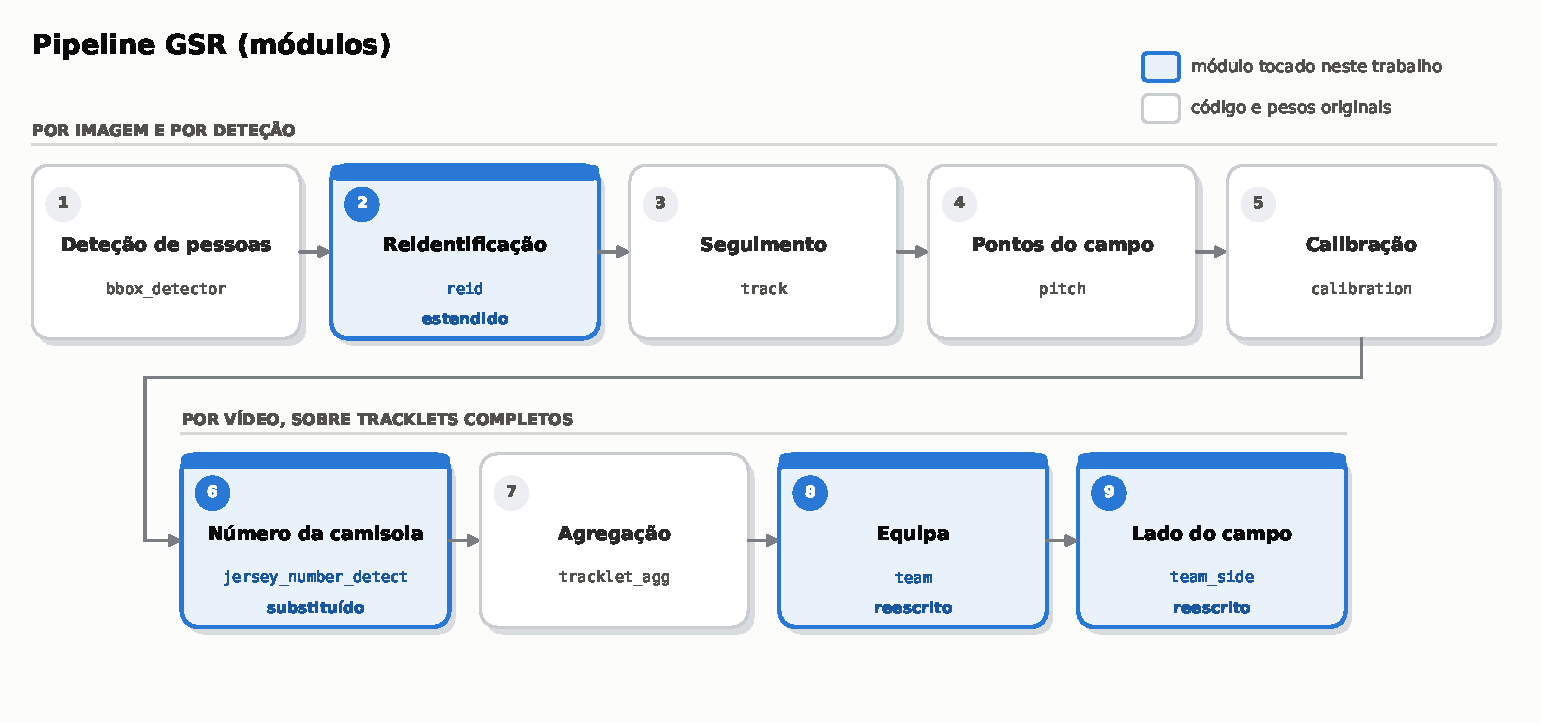
\includegraphics[width=\textwidth]{fig_pipeline_modulos.pdf}
    \caption{Os nove módulos do \emph{pipeline} da \emph{baseline}, pela ordem em que são executados.
    A azul, os quatro módulos em que este trabalho intervém. A reidentificação foi estendida com um
    descritor de cor, sem alterar o modelo nem a coluna de características original. A leitura do
    número de camisola foi substituída por um módulo novo. O agrupamento em equipas e a atribuição
    do lado do campo foram reescritos. Os restantes cinco módulos correm com o código e os pesos
    originais.}
    \label{fig:pipeline-modulos}
\end{figure}

Este trabalho intervém em quatro desses módulos. Três foram substituídos ou reescritos. Na
leitura do número de camisola, o OCR da \emph{baseline} deu lugar a um modelo multimodal de
visão e linguagem, descrito na Secção~\ref{sec:met-jnr}. Nos dois módulos da atribuição da equipa, o
agrupamento passou a ser auditado e o mapeamento para os lados passou a seguir uma cascata de
critérios, descritos na Secção~\ref{sec:met-equipa}. O quarto módulo, a reidentificação, foi
estendido e não alterado. O modelo e a coluna de características que alimenta o seguimento
mantêm-se intactos e acrescenta-se uma segunda coluna com um descritor de cor do equipamento,
calculado para cada deteção, que o módulo de agrupamento em equipas consome quando precisa. A deteção, o
seguimento, a calibração e a agregação por \emph{tracklet} correm com o código e os pesos
originais.

A escolha destes componentes não é arbitrária. São os que menos atenção têm recebido na
literatura, como evidencia a revisão do estado da arte, e aqueles em que a solução de referência
revela maior margem de melhoria, de forma particularmente acentuada no reconhecimento do número de
camisola. Isto torna-os o ponto de intervenção com maior retorno esperado.

Concentrar o esforço nestes módulos, em vez de o dispersar por todo o \emph{pipeline}, permitiu
estudá-los com uma profundidade que uma intervenção mais alargada dificilmente comportaria, em
linha com o âmbito de uma dissertação de mestrado. Isolá-los, mantendo tudo o resto inalterado,
garante que qualquer variação no desempenho final resulte diretamente das alterações introduzidas,
e não de uma reotimização global. Por serem independentes entre si, as alterações integram-se no
\emph{pipeline} sem exigir o reentreino das etapas anteriores, mantendo a compatibilidade direta
com a \emph{baseline} pública disponibilizada por \citet{somers2024soccernet}.

\section{Reconhecimento de Número de Camisola}\label{sec:met-jnr}

Na solução de referência, o reconhecimento dos números das camisolas baseia-se na biblioteca
MMOCR, que aplica um \emph{pipeline} genérico de deteção e reconhecimento de texto sobre o recorte de
cada jogador. Por atuar estritamente ao nível do carácter e sem incorporar conhecimento
\emph{a priori} sobre o domínio, esta abordagem trata o número como texto arbitrário e ignora
duas propriedades fundamentais do cenário desportivo.

A primeira é de cariz espacial. O número encontra-se numa região anatomicamente delimitada, a
zona dorsal do tronco, cuja localização pode ser estimada com precisão por um modelo de pose, em
vez de ser procurada de forma exaustiva em toda a imagem. A segunda é de cariz temporal. O mesmo
jogador é observado ao longo de múltiplos \emph{frames} consecutivos, e esta redundância,
frequentemente desaproveitada pelos métodos de inferência por \emph{frame} isolado, revela-se
crítica em situações de baixa resolução, oclusão parcial ou poses desfavoráveis.

Para tirar partido destas especificidades, o módulo proposto reorganiza a leitura numa sequência
de três fases interdependentes (Figura~\ref{fig:jnr-flow}). Inicialmente, um modelo de estimativa
de pose (YOLO26m-pose) extrai os pontos de interesse (\emph{keypoints}) do tronco e isola a
região dorsal, eliminando o fundo e as áreas irrelevantes do recorte. Em seguida, essa região é
processada por um modelo multimodal de visão e linguagem (\emph{Vision-Language Model}, VLM), o
Qwen2.5-VL, capaz de inferir conjuntamente sobre a informação visual e o contexto semântico do
equipamento e de distinguir o número de outros elementos gráficos ou patrocínios. Por fim, as
predições individuais associadas a cada \emph{tracklet} são consolidadas por um mecanismo de
votação temporal, convertendo uma sequência de inferências instantâneas numa decisão final mais
robusta e consistente.

\begin{figure}[htbp]
    \centering
    \includegraphics[width=\textwidth]{jnr_flow.png}
    \caption{Fluxo do módulo de reconhecimento do número de camisola. A estimativa de pose
    delimita a região dorsal, cujo recorte é interpretado pelo modelo multimodal Qwen2.5-VL
    quantizado a 4 bits. As leituras sucessivas de cada \emph{tracklet} são consolidadas por
    votação temporal numa decisão final única.}
    \label{fig:jnr-flow}
\end{figure}

\subsection{Recorte da Região Dorsal por Estimativa de Pose}

Para concentrar a leitura na zona onde o número efetivamente aparece, cada deteção é primeiro
processada por um modelo de estimativa de pose, o YOLO26m-pose. A partir dos \emph{keypoints} do
tronco, define-se uma região de interesse sobre as costas do jogador, alargada lateralmente para
acomodar variações de postura e enquadramento. Este recorte elimina o fundo, os membros e a zona
frontal, entregando ao modelo de leitura apenas o conteúdo relevante.

Antes de prosseguir, cada recorte passa por um filtro de qualidade que descarta os casos sem
informação utilizável. São rejeitados os recortes com dimensões inferiores a um limiar mínimo,
tipicamente jogadores muito distantes da câmara, e os recortes desfocados, quantificados pela
variância do Laplaciano. Este passo é determinante, uma vez que uma imagem sem resolução
suficiente não contém o número a ler e a sua submissão ao modelo apenas introduziria ruído. Ao
filtrar à entrada, garante-se que o modelo de leitura recebe somente recortes com hipótese real
de sucesso.

\subsection{Leitura por Modelo Multimodal de Visão e Linguagem}

O núcleo deste módulo assenta no modelo multimodal Qwen2.5-VL-3B-Instruct, responsável por
inferir e reportar o número a partir dos recortes da região dorsal de cada jogador. A opção por
uma arquitetura de visão e linguagem (\emph{Vision-Language Model}, VLM), em detrimento de um
motor de OCR dedicado, fundamenta-se na sua capacidade de interpretação contextual, que lhe
permite distinguir a numeração oficial de outros elementos gráficos presentes no equipamento,
como patrocínios, logótipos de marcas ou textos avulsos, que de outro modo introduziriam ruído.

A principal limitação prática derivou da infraestrutura computacional disponível, uma GPU móvel
equipada com apenas 6~GB de VRAM. Para viabilizar a execução dentro deste limite de memória, o
modelo foi carregado com quantização a 4 bits (\emph{4-bit quantization}), o que reduz a sua
ocupação de VRAM para aproximadamente 2~GB e assegura a sua coexistência com os restantes
módulos do \emph{pipeline}. Adicionalmente, para prevenir exceções de memória (\emph{out-of-memory})
durante as fases subsequentes de calibração, a instância do modelo é explicitamente libertada da
VRAM no término do processamento de cada vídeo.

A inferência do modelo foi moldada por engenharia de \emph{prompt}, assente em duas diretrizes
fundamentais:

\begin{enumerate}
    \item \textbf{Integridade estrutural da numeração.} O modelo é instruído a extrair a
    totalidade dos dígitos, prevenindo a omissão de um dígito inicial parcialmente ocluído, uma
    falha recorrente que tende a truncar números compostos, por exemplo classificando um 14 como
    4.
    \item \textbf{Política conservadora de recusa.} O modelo deve emitir uma resposta nula
    sempre que a amostra apresente baixa resolução, desfocagem acentuada ou ambiguidade visual,
    em vez de arriscar uma leitura incerta.
\end{enumerate}

Esta estratégia conservadora reflete uma decisão de projeto importante. No contexto da
reconstrução do estado de jogo e da métrica oficial do SoccerNet-GSR, a propagação de um erro de
classificação é significativamente mais penalizadora do que uma ausência temporária de leitura.
Por fim, para otimizar a eficiência das chamadas ao modelo, vários recortes do mesmo
\emph{tracklet} são apresentados na mesma \emph{prompt}. Este agrupamento é, contudo, limitado a
um número reduzido de \emph{tracklets} em cada chamada, de forma a respeitar o limiar a partir do
qual o mecanismo de atenção do modelo se satura e a precisão das respostas se degrada.

\subsection{Agregação Temporal por Votação}

A leitura efetuada sobre um recorte isolado é, por natureza, ruidosa. Uma pose desfavorável, uma
oclusão momentânea ou variações de iluminação são suficientes para induzir erros na inferência de
um \emph{frame}, mesmo quando a numeração se mantém globalmente legível ao longo do
\emph{tracklet} (Figura~\ref{fig:jnr-crops}). Para converter este conjunto de leituras individuais
numa decisão única e fiável, adotou-se um esquema de votação temporal estruturado em duas fases
hierárquicas, concebido para mitigar o ruído em diferentes escalas de tempo.

\begin{figure}[htbp]
    \centering
    \includegraphics[width=\textwidth]{jnr_crops_tracklet71.png}
    \caption{Recortes da região dorsal de um mesmo \emph{tracklet} ao longo do tempo. O número do
    jogador é nítido apenas em parte dos \emph{frames}, sendo comprometido nos restantes por
    desfoque, oclusão ou pose desfavorável. É esta variabilidade que justifica tanto o filtro de
    qualidade à entrada como a consolidação das leituras por votação temporal.}
    \label{fig:jnr-crops}
\end{figure}

Na primeira fase, os recortes de cada \emph{tracklet} são particionados em janelas temporais.
Cada janela apenas emite uma predição válida se uma fração dominante das suas leituras convergir
no mesmo valor, filtrando assim variações momentâneas e descartando instâncias erráticas entre
\emph{frames} adjacentes. Na segunda fase, a numeração final atribuída ao \emph{tracklet}
corresponde à hipótese mais votada entre as janelas, desde que cumpra uma quota mínima do total
emitido. Deste modo, a primeira fase filtra o ruído de alta frequência ao nível do \emph{frame},
enquanto a segunda arbitra leituras concorrentes que persistem no tempo, conferindo robustez ao
processo.

Um aspeto determinante deste mecanismo é a inclusão das leituras nulas no apuramento final, sendo
estas contabilizadas negativamente contra qualquer número candidato. Ao integrar as janelas sem
leitura no denominador da votação, impede-se que uma leitura incorreta e isolada, suportada por
uma única janela válida entre várias vazias, obtenha suporte suficiente para prevalecer. Esta
abordagem neutraliza o risco de falsos positivos decorrente do critério conservador do modelo de
visão, que gera deliberadamente uma elevada proporção de respostas nulas. A exigência de confiança
na inferência individual e a penalização da incerteza na agregação operam, assim, de forma
concertada, assegurando que a decisão final priorize a consistência temporal em detrimento de
evidências pontuais.

\subsection{Alternativas Consideradas}

A solução final para a leitura do número não foi imediata. Resultou da comparação de várias famílias
de OCR e de modelos de visão e linguagem, assim como de estratégias de pré-processamento da imagem.
A Tabela~\ref{tab:alternativas} resume as abordagens exploradas e a razão do seu descarte.

\begin{table}[htbp]
\centering
\caption{Alternativas de leitura do número consideradas e razão do seu descarte.}
\label{tab:alternativas}
\renewcommand{\arraystretch}{1.35}
\setlength{\tabcolsep}{6pt}
\begin{tabular}{|p{3.6cm}|p{9.0cm}|}
\hline
\textbf{Abordagem} & \textbf{Razão do descarte} \\
\hline
EasyOCR e OCR clássico &
Mesma limitação estrutural do MMOCR, falha em números pequenos ou inclinados e não
distingue o número de outros elementos gráficos. \\
\hline
PaddleOCR (com \emph{fine-tuning}) &
Falha de segmentação (\emph{segfault}) ao inicializar no mesmo processo que o CUDA do
\emph{pipeline}, e mesmo isolado não recuperou leituras face ao Qwen. \\
\hline
HunyuanOCR &
\emph{VLM} mais pesado, sem ganho de exatidão que compensasse o custo de VRAM e de
latência no \emph{hardware} disponível. \\
\hline
Qwen2.5-VL-7B &
Requer cerca de 10\,GB de VRAM, acima dos 6\,GB da GPU, o que inviabiliza a sua
utilização. \\
\hline
Super-resolução (RealESRGAN) &
A informação em falta não existe na imagem de origem, e a ampliação amplifica o ruído
em vez de a recuperar. \\
\hline
SAM-3D-Body &
Reconstrução tridimensional do corpo demasiado pesada para correr por \emph{frame} e
desadequada a um simples sinal de orientação. \\
\hline
Classificador de orientação &
O ganho de filtrar as \emph{frames} sem as costas visíveis não compensou, pois a votação
por \emph{tracklet} já absorve naturalmente essas \emph{frames}. \\
\hline
\end{tabular}
\end{table}


Estas experiências convergem numa conclusão. Em condições de baixa resolução, o fator decisivo não é
a escolha do motor de OCR mais potente, mas sim entregar ao modelo a imagem certa, o recorte da
região dorsal obtido por pose, e agregar bem as leituras ao longo do tempo. O Qwen2.5-VL-3B foi
escolhido pelo equilíbrio entre exatidão e ocupação de memória, e não por ser o modelo de maior
dimensão.

\section{Atribuição da Equipa e do Lado do Campo}\label{sec:met-equipa}

Atribuir a equipa a um jogador é responder a duas perguntas distintas. A primeira é com quem
ele joga, e resolve-se separando os \emph{tracklets} do vídeo em dois grupos. A segunda é qual
dos dois grupos defende a baliza da esquerda e qual defende a da direita, porque é assim que a
anotação do SoccerNet-GSR identifica as equipas, por \emph{left} e \emph{right}, e não por
nome ou por cor. Um erro em qualquer das duas perguntas conta como erro na atribuição da equipa.

A solução de referência responde às duas perguntas de forma muito simples. Para a primeira,
calcula a média das características de reidentificação de cada \emph{tracklet} com função de
jogador, um vetor de 256 dimensões produzido pelo PRTreID, e aplica-lhe um \emph{k-means} com
dois grupos. O \emph{k-means} é um algoritmo de agrupamento não supervisionado que reparte as
observações num número fixo de grupos, atribuindo cada observação ao centro mais próximo e
recalculando os centros até a partição estabilizar. Para a segunda pergunta, calcula a média da
coordenada horizontal no campo de todas as deteções de cada grupo e declara \emph{right} o grupo
cuja média está mais à direita. Os guarda-redes ficam de fora do agrupamento e recebem o lado
da metade do campo em que se encontram. Nada disto é auditado. Se o \emph{k-means} misturar as
equipas, ou se a média da posição apontar para o lado errado, o erro propaga-se a todos os
\emph{tracklets} do vídeo.

Foi exatamente isso que a medição da solução de referência revelou, e que o Capítulo~\ref{cap:resultados}
quantifica. A esmagadora maioria dos \emph{tracklets} mal atribuídos não vinha de grupos
misturados mas de grupos corretos mapeados ao lado errado, em vídeos inteiros a $0\%$. As
alterações descritas a seguir atacam por isso os dois momentos do processo, mas com prioridades
diferentes. No agrupamento, mantém-se o método original e acrescenta-se uma auditoria com uma
alternativa baseada na cor do equipamento, que exige um descritor novo calculado na
reidentificação. No mapeamento para os lados, substitui-se a comparação de médias por uma cascata
de quatro critérios que só recorre a essa comparação em último lugar.

\subsection{Descritor de Cor do Equipamento}\label{sec:descritor-cor}

As características de reidentificação são treinadas para distinguir indivíduos, não equipas. Dois
jogadores da mesma equipa ficam próximos nesse espaço porque partilham o equipamento, mas quando
os dois equipamentos são parecidos, ou quando a iluminação e a resolução degradam a imagem, a
distância entre equipas deixa de ser maior do que a distância entre jogadores da mesma equipa. Para
dispor de um sinal que dependa apenas da cor da camisola, acrescentou-se ao módulo de
reidentificação o cálculo de um descritor de cor por deteção, ilustrado na
Figura~\ref{fig:descritor-cor}.

\begin{figure}[htbp]
    \centering
    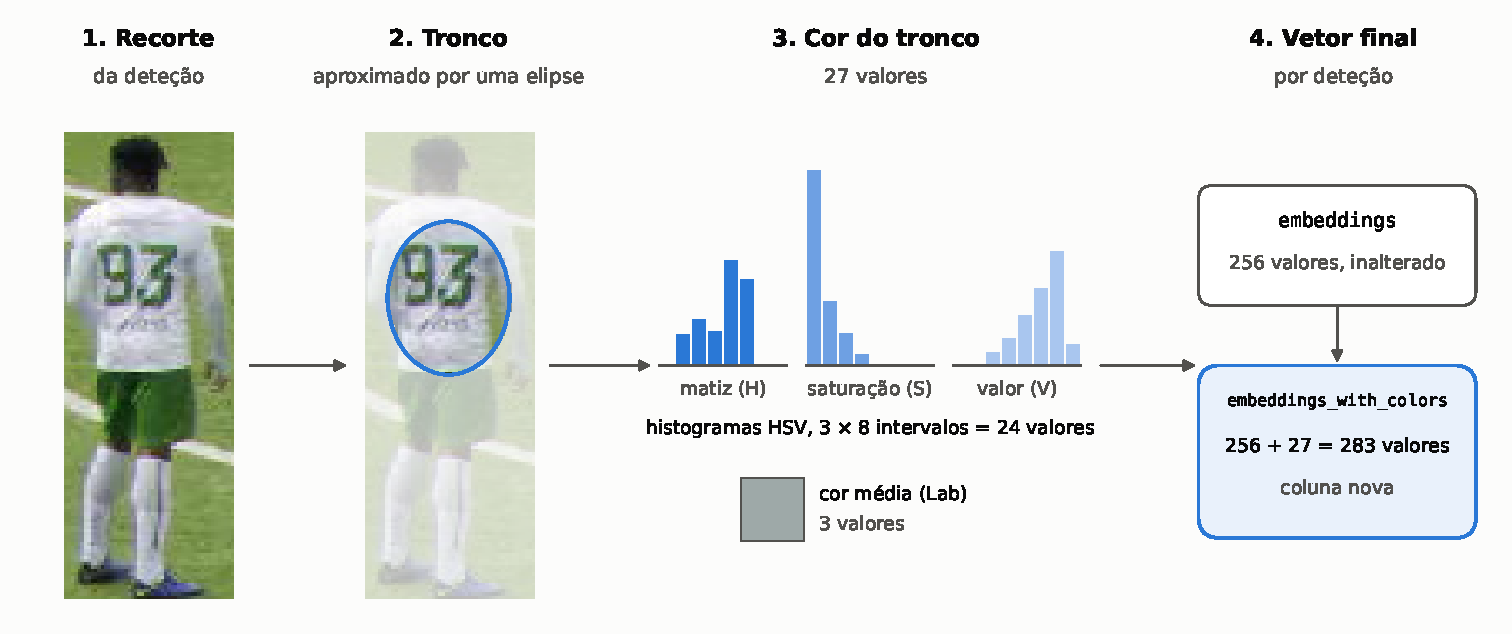
\includegraphics[width=\textwidth]{fig_descritor_cor.pdf}
    \caption{Construção do descritor de cor do equipamento para uma deteção real (vídeo SNGS-116,
    primeira imagem, caixa da anotação). A máscara do torso está desenhada em esquema, porque o
    mapa de atenção do BPBreID não é guardado. Da esquerda para a direita, o recorte da deteção, a
    região do torso, os píxeis selecionados, os três histogramas HSV de oito classes, a cor média
    Lab e o vetor final, que junta os 27 valores de cor às 256 características de reidentificação
    numa coluna nova, deixando a coluna original intacta.}
    \label{fig:descritor-cor}
\end{figure}

O descritor é calculado sobre o torso e não sobre o recorte inteiro. O PRTreID assenta no BPBreID,
um modelo de reidentificação por partes do corpo que produz, para cada deteção, um mapa de atenção
por parte, e uma dessas partes é o torso. Esse mapa é redimensionado ao tamanho do recorte,
normalizado pelo seu máximo, e os píxeis com atenção igual ou superior a $0.25$ formam a máscara.
Isto exclui a relva, a pele, os calções e as meias, que teriam cores próprias e iguais nas duas
equipas. Quando a máscara reúne menos de $16$ píxeis, o que acontece em deteções muito pequenas ou
truncadas, usa-se em alternativa a banda central do recorte, entre $25\%$ e $75\%$ da altura.

Sobre os píxeis selecionados calculam-se duas coisas. A primeira é um histograma por canal no
espaço HSV, com oito classes por canal, cada um normalizado para somar um, o que dá $24$ valores.
A matiz capta a cor dominante da camisola de forma pouco sensível ao brilho. A saturação e o valor
captam os equipamentos brancos, pretos ou cinzentos, que não têm matiz definida e que só se
distinguem por estes dois canais. A segunda é a cor média dos mesmos píxeis no espaço Lab,
normalizada ao intervalo $[0,1]$, mais três valores, que resume a cor num espaço percetualmente
uniforme e complementa o histograma nos casos em que a camisola combina duas cores. Os $27$ valores
resultantes são concatenados às $256$ características de reidentificação e guardados numa coluna
nova, \texttt{embeddings\_with\_colors}, com $283$ dimensões. A coluna original,
\texttt{embeddings}, não é tocada, pelo que o seguimento, que a consome, corre exatamente como na
\emph{baseline}. O módulo de agrupamento em equipas é o único consumidor da coluna nova e usa dela apenas os $27$
valores finais.

\subsection{Agrupamento em Duas Equipas com Auditoria}\label{sec:agrupamento}

O agrupamento parte do mesmo ponto que a solução de referência. Para cada \emph{tracklet} com
função de jogador calcula-se a média das suas deteções em três grandezas, o vetor de
reidentificação de $256$ dimensões, o descritor de cor de $27$ dimensões e a coordenada
horizontal no campo, esta última ignorando as deteções projetadas fora do relvado, com $|x|$ acima
de $52.5$ metros, que resultam de falhas pontuais de calibração. Aplica-se o \emph{k-means} com
dois grupos ao vetor de reidentificação, com dez inicializações para reduzir a dependência do
ponto de partida. A aparência aprendida é o sinal principal, porque quando funciona é mais
discriminativo do que a cor, e por isso é sempre calculado primeiro.

A diferença está no que se faz a seguir. Antes de aceitar esta partição, medem-se duas grandezas
que descrevem a sua qualidade. A primeira é o coeficiente de silhueta médio. Para cada
\emph{tracklet}, compara a distância média aos elementos do seu grupo com a distância média aos
elementos do outro grupo, e resume a relação num valor entre $-1$ e $1$. Valores próximos de $1$
indicam grupos compactos e afastados, valores próximos de zero indicam grupos que se sobrepõem. A
segunda é a distância euclidiana entre os centros dos dois grupos no espaço de reidentificação.
Com estas duas grandezas, a partição é rejeitada quando qualquer um de dois gatilhos dispara.

O gatilho A é a silhueta. Quando o coeficiente médio fica abaixo de $0.28$, os dois grupos não
estão separados o suficiente para se confiar que correspondam às duas equipas. O gatilho B é
herdado de uma iteração anterior do módulo e combina duas condições. A jogada tem de estar
concentrada numa das metades do campo, com pelo menos $85\%$ dos \emph{tracklets} com posição
válida do mesmo lado da linha de meio-campo, e os centros dos dois grupos têm de estar a menos de
$2.04$ de distância no espaço de reidentificação. A primeira condição identifica os vídeos em que
a posição não vai ajudar a decidir o lado, e nos quais um erro de agrupamento seria mais
penalizador. A segunda identifica grupos pouco afastados. Importa dizer claramente de onde vem o
valor $2.04$. Nos quatro vídeos do conjunto de teste em que este gatilho dispara, a distância
entre centros foi de $1.799$, $1.896$, $1.981$ e $2.035$, e o limiar ficou $0.005$ acima do maior
destes valores. É um limiar ajustado a esses casos, e não uma constante com significado
geral. Foi mantido porque a sua remoção introduzia regressões no conjunto de teste, e o gatilho A,
introduzido mais tarde, foi calibrado sobre os conjuntos de teste e de validação em conjunto
precisamente para cobrir os casos em que o gatilho B, por exigir a concentração numa metade, nunca
disparava.

Quando um dos gatilhos dispara, repete-se o \emph{k-means} com dois grupos, agora sobre os $27$
valores do descritor de cor, normalizados por dimensão para média zero e desvio-padrão um. O
descritor é usado sozinho, e não concatenado ao vetor de reidentificação, por uma razão
concreta. Com a normalização por dimensão, cada uma das $283$ dimensões pesa o mesmo, e as $256$ da
reidentificação abafam as $27$ da cor, e a partição pouco se afasta da original. A partição por cor é depois submetida a uma guarda de
degenerescência. O grupo menor tem de reunir pelo menos $20\%$ dos \emph{tracklets}. Se não
reunir, o \emph{k-means} separou provavelmente um punhado de deteções atípicas, com sombra ou
oclusão, do resto, e não as duas equipas. Nesse caso mantém-se a partição por reidentificação.
Esta guarda só se aplica quando foi o gatilho A a disparar. Quando é o gatilho B, a partição por
cor é aceite sem a guarda, para preservar o comportamento validado da regra herdada. A
Figura~\ref{fig:team_cluster} mostra, para um vídeo real, a separação dos dois grupos no espaço de
reidentificação e no descritor de cor.

A frequência com que cada ramo é tomado dá a medida do papel da auditoria. Nos $57$ vídeos de
treino, o agrupamento por reidentificação foi mantido em $49$ e a cor foi usada em $8$, sete deles
pelo gatilho B e um apenas pelo gatilho A. A guarda de degenerescência recusou a cor uma vez. Nos
$39$ vídeos de teste com estado guardado, a cor foi usada em $4$. Ou seja, em mais de $85\%$ dos
vídeos o agrupamento é exatamente o da solução de referência. A auditoria intervém numa minoria de
casos e é nessa minoria que o descritor de cor tem de ser melhor do que a reidentificação.

\begin{figure}[htbp]
    \centering
    \includegraphics[width=\textwidth]{team_cluster_space.png}
    \caption{Agrupamento dos \emph{tracklets} de um vídeo nas duas equipas. À esquerda, a projeção
    das características de reidentificação em duas dimensões, onde o \emph{k-means} separa os dois
    grupos com um coeficiente de silhueta de $0.42$. À direita, o descritor de cor da camisola dos
    mesmos \emph{tracklets}, que preserva a separação, com silhueta de $0.32$, e serve de alternativa
    quando a reidentificação é pouco fiável.}
    \label{fig:team_cluster}
\end{figure}

\subsection{Mapeamento para os Lados do Campo}\label{sec:mapeamento}

Definidas as duas equipas, resta dizer qual delas é \emph{left} e qual é \emph{right}, isto é,
qual tem a sua baliza à esquerda da imagem e qual a tem à direita. A única informação disponível
para o fazer é a posição dos jogadores no relvado, projetada pela calibração, porque a aparência
não diz nada sobre a baliza que uma equipa defende. A suposição de base, comum à solução de
referência e aos quatro critérios descritos a seguir, é a de que os jogadores de uma equipa estão,
em média, mais perto da sua própria baliza do que os adversários, porque é junto dela que tem os
defesas e o guarda-redes. Logo, a equipa cujos jogadores estão mais à direita é a que defende a
baliza da direita. Tudo o que se segue são formas, cada vez menos exigentes, de aplicar esta
suposição, e o exemplo no fim da secção mostra o que acontece quando ela não se verifica. A
solução de referência usa a posição da forma mais direta, comparando a média da coordenada horizontal
de todas as deteções de cada grupo. Esta comparação tem três fraquezas que a medição tornou
evidentes. Uma única deteção projetada a centenas de metros do campo, por uma falha momentânea da
calibração, desloca a média do seu grupo. As deteções de um jogador que aparece durante todo o
clip pesam muito mais do que as de um jogador que aparece pouco, e a média reflete quem esteve mais
tempo em cena, não onde a equipa está. E, sobretudo, quando as duas equipas estão na mesma metade
do campo, o que acontece em qualquer lance junto de uma baliza, as duas médias distam poucos
metros e a sua ordem não tem relação com a baliza que cada equipa defende.

O mapeamento passou a seguir uma cascata de quatro critérios, aplicados por ordem até um deles
decidir, resumida na Figura~\ref{fig:cascata-lado}. Em todos eles as deteções com $|x|$ acima de
$60$ metros são descartadas, o que elimina a primeira fraqueza. Os dois primeiros critérios contam
\emph{tracklets} e não deteções, o que atenua a segunda.

\begin{figure}[htbp]
    \centering
    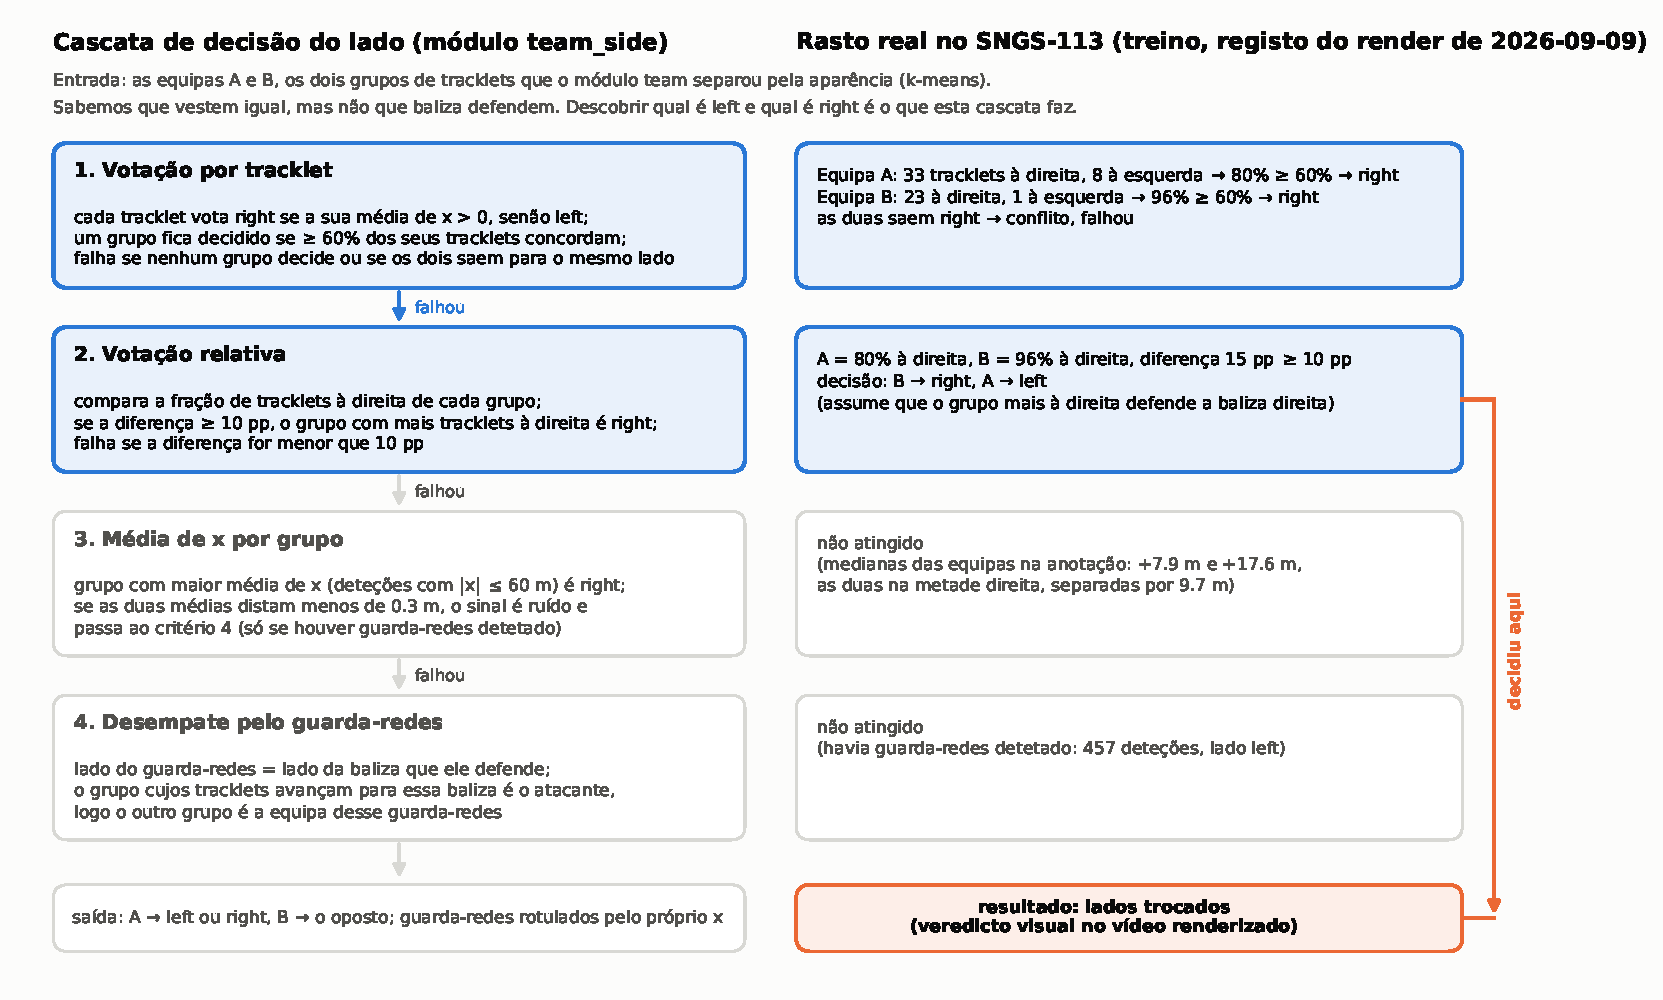
\includegraphics[width=\textwidth]{fig_cascata_lado.pdf}
    \caption{À esquerda, os quatro critérios da cascata que atribui cada grupo ao seu lado do
    campo, aplicados por ordem até um deles decidir. À direita, o rasto real da cascata no vídeo
    SNGS-113 do conjunto de treino, extraído do registo de execução. As duas equipas saem ambas
    \emph{right} da votação por \emph{tracklet}, a votação relativa decide com uma diferença de
    $15$ pontos percentuais e o resultado é o mapeamento invertido. Os critérios seguintes, incluindo
    o que consulta o guarda-redes, nunca são atingidos.}
    \label{fig:cascata-lado}
\end{figure}

O primeiro critério é uma votação por \emph{tracklet}. Cada \emph{tracklet} vota \emph{right} se
a sua posição média está à direita da linha de meio-campo e \emph{left} caso contrário. Um grupo
fica decidido quando pelo menos $60\%$ dos seus \emph{tracklets} votam no mesmo lado. Se só um
dos grupos ficar decidido, o outro recebe o lado oposto. O critério falha em duas situações,
quando nenhum grupo atinge a maioria e quando os dois grupos ficam decididos para o mesmo lado.
Esta segunda situação é frequente e corresponde precisamente ao caso em que a jogada decorre numa
só metade do campo.

O segundo critério é uma votação relativa. Calcula-se, para cada grupo, a fração dos seus
\emph{tracklets} com posição média à direita do meio-campo, exigindo pelo menos três
\emph{tracklets} por grupo. Se a diferença entre as duas frações for de pelo menos $10$ pontos
percentuais, o grupo com maior fração recebe \emph{right}. A hipótese subjacente é a de que,
mesmo com as duas equipas na mesma metade, a equipa que defende a baliza direita tende a estar
mais perto dela. É uma hipótese razoável na maioria dos lances, mas não é uma lei, e o exemplo
abaixo mostra um caso em que falha.

O terceiro critério é a comparação de médias da solução original, com o filtro de $60$ metros. O
grupo com maior média recebe \emph{right}. O quarto só é consultado quando o terceiro não tem
sinal, isto é, quando as duas médias distam menos de $0.3$ metros, e apenas se houver um
guarda-redes detetado. Nesse caso, mede-se em cada \emph{tracklet} com pelo menos dez imagens o
deslocamento líquido ao longo do clip, a diferença entre a última e a primeira posição, e
calcula-se a média por grupo, com sinal positivo na direção da baliza onde está o guarda-redes.
O grupo que mais avança para essa baliza é o que a ataca, logo é a equipa do lado oposto, e o
outro grupo é a equipa desse guarda-redes. Os guarda-redes, tal como na solução de referência,
recebem diretamente o lado da metade em que se encontram. Uma quinta heurística, que tomava o grupo
mais próximo de uma baliza numa bola parada como o atacante, foi experimentada e removida. Nos $39$
vídeos de teste disparou uma vez e errou, porque o grupo que se aglomera junto de uma baliza é,
pelo menos tantas vezes, a equipa que a defende.

Três casos reais, resumidos na Figura~\ref{fig:cascata-exemplos}, mostram a cascata a decidir em
pontos diferentes. Em todos eles, A e B são as duas equipas que saem do agrupamento, das quais só
se sabe que vestem igual.

O primeiro é o caso comum. No vídeo SNGS-060 do conjunto de treino o jogo está aberto, com as duas
equipas repartidas pelas duas metades. Na votação por \emph{tracklet}, a equipa A tem $15$
\emph{tracklets} na metade direita e $19$ na esquerda, $44\%$ à direita, e a equipa B tem $22$ e
$20$, $52\%$. Nenhuma chega aos $60\%$ num sentido nem no outro, pelo que nenhuma fica decidida e o
critério falha. Na votação relativa, a diferença entre $52\%$ e $44\%$ é de $8$ pontos, abaixo dos
$10$ exigidos, e o critério também falha. Na média de x, A está a $-2.0$ metros e B a $+2.4$, uma
distância de $4.4$ metros, muito acima dos $0.3$ que marcam a ausência de sinal. B recebe
\emph{right} e A recebe \emph{left}. A verificação visual confirma o resultado. É o percurso da
maioria dos vídeos, e mostra que os dois primeiros critérios só decidem quando a distribuição das
equipas pelas metades é clara.

O segundo caso mostra o guarda-redes a decidir. No vídeo SNGS-195 do conjunto de teste o jogo
decorre inteiro na metade esquerda. A equipa A tem $4$ \emph{tracklets} à direita e $16$ à
esquerda, $80\%$ à esquerda, e a equipa B tem $5$ e $30$, $86\%$. As duas ultrapassam os $60\%$ e
as duas saem \emph{left}, o que é um conflito, e o critério falha. Na votação relativa, $20\%$
contra $14\%$ à direita dá uma diferença de $6$ pontos, insuficiente. Na média de x, A está a
$-23.03$ metros e B a $-23.04$, uma distância de $0.01$ metros. Não há sinal nenhum na posição, e
é aqui que o quarto critério entra. Há um guarda-redes detetado junto da baliza esquerda, com $315$
deteções a $x \approx -46$ metros. Mede-se então quanto cada equipa avançou para essa baliza ao
longo do clip. A equipa A avançou em média $1.4$ metros e a equipa B $5.8$ metros. B é a que
mais avança para a baliza esquerda, logo é a que a ataca, logo a sua baliza é a direita. B recebe
\emph{right} e A recebe \emph{left}, e os $31$ \emph{tracklets} do vídeo ficam corretos. Este
vídeo estava a $0\%$ antes de o quarto critério existir, porque a comparação de médias decidia ao
acaso sobre uma diferença de um centímetro.

O terceiro caso, o vídeo SNGS-113 do conjunto de treino, mostra como a cascata decide e onde a
hipótese do segundo critério se quebra. A Figura~\ref{fig:113-campo} mostra a anotação de referência sobre o
campo. As duas equipas estão inteiras na metade direita, com as medianas a $+7.9$ e $+17.6$ metros,
apenas $9.7$ metros uma da outra, enquanto os dois guarda-redes estão a $73.5$ metros um do outro.
O rasto do registo de execução, na Figura~\ref{fig:cascata-lado}, diz o que a cascata fez com estes
dados. Chamem-se A e B às duas equipas que saem do agrupamento, das quais nesta altura só se
sabe que vestem igual, e não que baliza defendem. Na votação por \emph{tracklet}, a equipa A
teve $33$ votos \emph{right} e $8$ \emph{left}, $80\%$, e a equipa B teve $23$ e $1$, $96\%$.
Ambas ultrapassaram os $60\%$ e ambas saíram \emph{right}, pelo que o critério falhou. Na
votação relativa, a diferença entre $96\%$ e $80\%$ foi de $15$ pontos, acima dos $10$ exigidos,
e B recebeu \emph{right}. A verificação visual do
vídeo mostrou que estava invertido. A diferença entre $80\%$ e $96\%$ é a diferença entre oito e um
\emph{tracklets} do lado esquerdo, num conjunto de $65$ \emph{tracklets} para cerca de vinte
jogadores. São fragmentos de trajetórias e não jogadores, e um jogador cuja trajetória o seguimento
partiu em vários pedaços pesa várias vezes. Com as duas equipas na mesma metade, esta diferença
não é um sinal do lado, é ruído de fragmentação. Ao mesmo tempo, o sinal que decidiria sem
ambiguidade, o guarda-redes, com $73.5$ metros de separação, está na cascata, mas no último lugar,
e o segundo critério decidiu antes de ele ser consultado.

\begin{figure}[htbp]
    \centering
    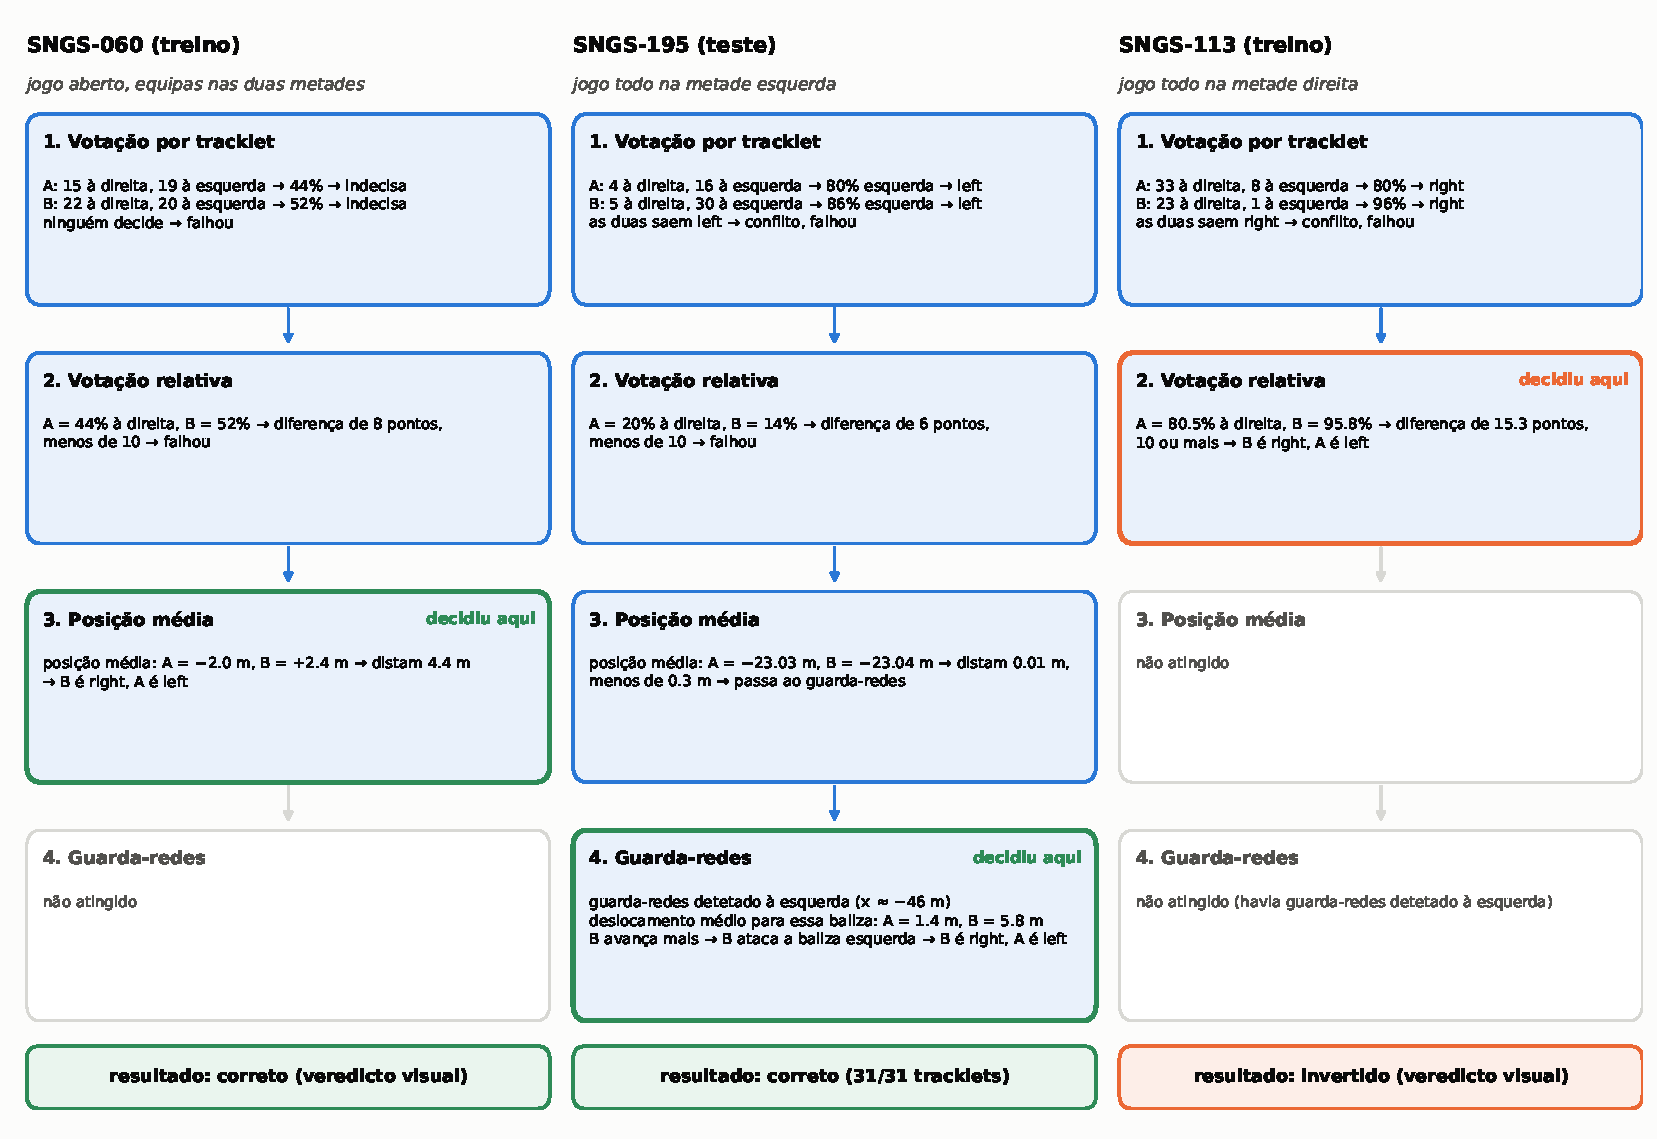
\includegraphics[width=\textwidth]{fig_cascata_exemplos.pdf}
    \caption{A cascata do lado em três vídeos reais. À esquerda, SNGS-060, jogo aberto, decidido
    pela média de x no terceiro critério. Ao centro, SNGS-195, jogo inteiro na metade esquerda com
    as médias das duas equipas a um centímetro, decidido pelo guarda-redes no quarto critério. À
    direita, SNGS-113, jogo inteiro na metade direita, decidido pela votação relativa no segundo
    critério, com o resultado invertido. Os valores do SNGS-060 e do SNGS-113 vêm dos registos de
    execução; os do SNGS-195 vêm da reexecução dos módulos de equipa sobre o estado guardado.}
    \label{fig:cascata-exemplos}
\end{figure}

\begin{figure}[htbp]
    \centering
    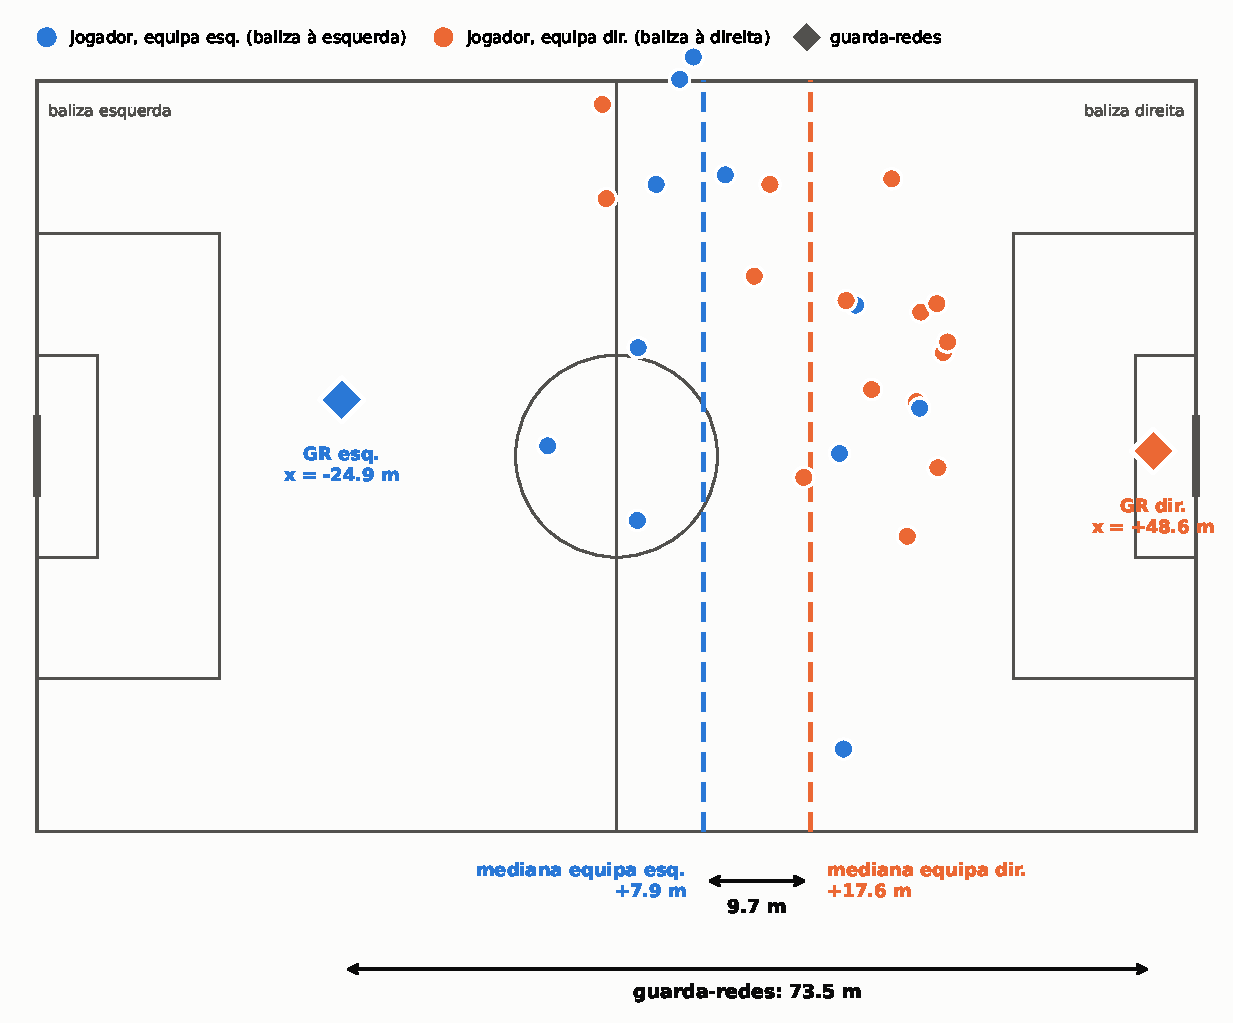
\includegraphics[width=0.9\textwidth]{fig_113_campo.pdf}
    \caption{Anotação de referência do vídeo SNGS-113 sobre o campo, com um marcador por trajetória
    anotada na sua posição mediana ao longo dos $30$ segundos do clip. As duas equipas estão na
    metade direita e as suas medianas distam $9.7$ metros. Os guarda-redes distam $73.5$ metros. Os
    critérios 1 a 3 da cascata usam apenas a posição dos jogadores, o critério 4 é o único que
    consulta o guarda-redes.}
    \label{fig:113-campo}
\end{figure}

Este caso não é isolado no que revela, e importa ler os números com honestidade. Nos $57$ vídeos
de treino, a decisão saiu do primeiro critério em $17$, do segundo em $12$, do terceiro em $28$ e
do quarto em nenhum. Nos $39$ vídeos de teste com estado guardado, saiu do primeiro em $5$, do
terceiro em $33$ e do quarto em $1$. Isto é, na maioria dos vídeos a decisão continua a vir da
comparação de médias da solução original, agora protegida pelo filtro de $60$ metros, e as duas
votações decidem quando os grupos estão claramente em metades diferentes ou com uma assimetria de
pelo menos $10$ pontos. Em que vídeos o novo mapeamento corrige a solução original é o que o
Capítulo~\ref{cap:resultados} mede, vídeo a vídeo. O guarda-redes, que é o sinal mais robusto para esta
decisão porque não acompanha as fases de ataque, continua a ser consultado em último lugar, e a
sua promoção na cascata fica identificada como a alteração de maior potencial ainda por fazer.

Os limiares da cascata foram recalibrados em conjunto sobre os dados de teste e de validação. A
maioria exigida na votação é de $0.60$. A diferença mínima da votação relativa desceu de $0.25$
para $0.10$ e a distância mínima entre médias desceu de $0.5$ para $0.3$ metros. A recalibração
obedeceu a uma condição estrita, a de não degradar nenhum vídeo do conjunto de teste que já
estivesse correto, de modo que cada ajuste só foi aceite quando resolvia casos falhados sem
introduzir novas falhas.

\FloatBarrier

\section{Ambiente Experimental}

Esta secção descreve as condições em que o sistema foi desenvolvido e avaliado. Apresenta o ambiente
computacional e o conjunto de dados, enumera os hiperparâmetros que governam os módulos
intervencionados e define o protocolo de avaliação sobre o qual assentam os resultados do capítulo
seguinte.

\subsection{Ambiente Computacional e Conjunto de Dados}

Todo o trabalho foi implementado com base no \emph{framework} TrackLab, responsável pela gestão e
execução sequencial dos módulos do \emph{pipeline}, tendo como suporte a biblioteca PyTorch. O
desenvolvimento decorreu em Python~3.10; a avaliação final, tanto do sistema proposto como da
solução de referência, correu num único ambiente em Python~3.12, com as versões das bibliotecas
fixadas, de modo que os dois sistemas são comparados nas mesmas condições.
A principal restrição computacional decorreu da infraestrutura de \emph{hardware}
disponível, um sistema portátil equipado com uma GPU NVIDIA RTX~3060 com apenas 6~GB de VRAM. Esta
limitação condicionou várias das decisões metodológicas adotadas, com destaque para a quantização a
4 bits do modelo de visão e linguagem, com recurso à biblioteca \emph{bitsandbytes}, e a desalocação
manual da memória de vídeo após o processamento de cada sequência.

A validação experimental utilizou o conjunto de dados SoccerNet-GSR, constituído por
sequências de vídeo anotadas e divididas nos subconjuntos de treino, validação e teste.
O protocolo de avaliação abrangeu a totalidade das 160 sequências anotadas,
correspondentes aos conjuntos de treino (57 vídeos), de validação (54 vídeos) e de teste
(49 vídeos); uma sequência do conjunto de validação (SNGS-096) não pôde ser processada por
uma falha do módulo de calibração, comum aos dois sistemas, pelo que a comparação incide
sobre 159 vídeos. Para cada interveniente, este conjunto disponibiliza a anotação de
referência (\emph{ground truth}) da posição no terreno de jogo, da equipa, da função e do
número de camisola, permitindo tanto a avaliação integrada do sistema como o teste
isolado de cada módulo.

O papel de cada subconjunto neste trabalho difere do habitual e convém precisá-lo. Nenhum dos
módulos desenvolvidos envolve treino de modelos, pelo que o subconjunto de treino não foi usado
para aprender parâmetros. Os limiares de decisão foram afinados sobre os conjuntos de teste e de
validação, como se descreve na Secção~\ref{sec:mapeamento}, e o conjunto de treino permaneceu
inteiramente por observar até à fase final. Serve, por isso, o propósito de um conjunto de
retenção, ou seja, de medir o desempenho em dados que não intervieram em nenhuma decisão de
conceção.

\subsection{Parametrização dos Módulos}

O comportamento dos módulos desenvolvidos é definido por um conjunto de hiperparâmetros, resumidos na
Tabela~\ref{tab:hiperparametros}. Os valores relativos ao reconhecimento do número de camisola foram
definidos por experimentação, procurando equilibrar a fiabilidade da leitura com o custo
computacional, ao passo que os limiares da atribuição da equipa e do lado do campo resultam da
recalibração descrita na Secção~\ref{sec:mapeamento}, conduzida sobre os conjuntos de teste e de
validação.


\begin{table}[htbp]
    \centering
    \caption{Hiperparâmetros dos módulos intervencionados e respetiva função.}
    \label{tab:hiperparametros}
    \begin{tabular}{lll}
        \hline
        \textbf{Parâmetro} & \textbf{Valor} & \textbf{Função} \\
        \hline
        \multicolumn{3}{l}{\emph{Reconhecimento de número de camisola (pose e recorte)}} \\
        Confiança da pose            & $0.25$          & Deteção mínima dos \emph{keypoints} \\
        Alargamento lateral da ROI   & $0.55$          & Margem lateral sobre o tronco \\
        Margem superior da ROI       & $0.10$          & Recorte acima dos ombros \\
        Fração de altura do tronco   & $0.90$          & Extensão vertical da região dorsal \\
        \hline
        \multicolumn{3}{l}{\emph{Reconhecimento de número de camisola (filtro de qualidade)}} \\
        Dimensão mínima do recorte   & $25\times30$~px & Rejeita jogadores distantes \\
        Nitidez mínima               & $40.0$          & Variância do Laplaciano \\
        \hline
        \multicolumn{3}{l}{\emph{Reconhecimento de número de camisola (leitura e votação)}} \\
        Modelo de leitura            & Qwen2.5-VL-3B (4 bits) & Inferência do número \\
        \emph{Tracklets} por chamada & $4$             & Agrupamento de chamadas ao modelo \\
        Recortes por chamada         & $20$            & Limite antes de saturar a atenção \\
        Concordância na janela       & $0.75$          & Consenso dentro de cada janela \\
        Concordância no \emph{tracklet} & $0.45$       & Consenso entre janelas, com nulos \\
        \hline
        \multicolumn{3}{l}{\emph{Descritor de cor (reidentificação)}} \\
        Atenção mínima do torso      & $0.25$          & Fração do máximo do mapa BPBreID \\
        Píxeis mínimos da máscara    & $16$            & Abaixo, usa a banda central \\
        Classes por canal HSV        & $8$             & Três canais, $24$ valores \\
        \hline
        \multicolumn{3}{l}{\emph{Atribuição da equipa (agrupamento)}} \\
        Limiar de silhueta           & $0.28$          & Abaixo, recorre à cor da camisola \\
        Concentração num dos lados   & $0.85$          & Condição do teste complementar \\
        Distância entre centros      & $2.04$          & Abaixo, separação por ReID frágil \\
        Fração mínima do grupo menor & $0.20$          & Aceitação da alternativa de cor \\
        Dimensão do descritor de cor & $27$            & $24$ do histograma HSV e $3$ da média Lab \\
        Posição válida (agrupamento) & $|x| \le 52.5$~m & Ignora projeções fora do relvado \\
        \hline
        \multicolumn{3}{l}{\emph{Atribuição da equipa (lado do campo)}} \\
        Posição válida (lado)        & $|x| \le 60$~m   & Descarta artefactos de calibração \\
        Maioria na votação           & $0.60$          & Fração dominante por \emph{tracklet} \\
        Diferença relativa mínima    & $0.10$          & Margem do voto relativo \\
        Distância mínima entre médias & $0.3$~m        & Abaixo, aciona o desempate pelo guarda-redes \\
        Imagens mínimas por \emph{tracklet} & $10$    & Para medir o deslocamento no desempate \\
        \hline
    \end{tabular}
\end{table}


\subsection{Protocolo de Avaliação}

A avaliação é conduzida em dois níveis complementares, seguindo a lógica exposta na
Secção~\ref{sec:metricas}. Ao nível do sistema completo, o desempenho é medido pela métrica oficial
do desafio, o GS-HOTA, calculada com a implementação oficial (TrackEval) sobre cada subconjunto
inteiro. Para separar o contributo de cada atributo, a métrica é ainda calculada com os atributos
ativados de forma progressiva, primeiro apenas a posição, depois a função, a equipa e o número de
camisola, o que permite imputar a cada módulo a parcela da métrica que lhe cabe. Ao nível de cada
módulo intervencionado mede-se a exatidão por \emph{tracklet} da leitura do número de camisola e da
atribuição da equipa e do lado, por comparação direta com a anotação de referência.

O termo de comparação é a solução de referência executada por nós, nos mesmos 159 vídeos e no mesmo
ambiente, com os seus módulos originais, incluindo o leitor de números MMOCR. Como a deteção, o
seguimento e as representações de reidentificação são partilhados, os \emph{tracklets} avaliados são
os mesmos nos dois sistemas e qualquer diferença resulta apenas dos módulos alterados. As métricas
automáticas são complementadas por uma inspeção visual dos 159 vídeos de cada sistema, na qual cada
sequência é classificada numa de cinco categorias: correta; lado trocado; agrupamento colapsado numa
só equipa; agrupamento misturado; e uma equipa inteira classificada como equipa de arbitragem. Esta
inspeção serve para caracterizar os erros que a métrica agrega e para identificar as sequências em
que a própria anotação de referência está invertida.

A recalibração dos limiares seguiu um protocolo estrito de ausência de regressões. Cada ajuste foi
testado em simultâneo nos conjuntos de teste e de validação e só foi aceite quando corrigia casos
anteriormente falhados sem degradar nenhum vídeo já correto. Deste modo, garante-se que os ganhos
reportados no capítulo seguinte resultam de melhorias consistentes em todo o conjunto avaliado, e não
de um sobreajuste a casos particulares.